\chapter{3-Gems}
\label{chap:gems}

\section{Definition}

An {\em $(n+1)$-graph} is a regular graph where all its vertices
have degree $n+1$ and the edges incident to each vertex have
distinct colors $0,1,\ldots,n$. Let $K \subseteq \{0,1,\ldots,n\}$
be a subset of colors and $G$ an $(n+1)$-graph. Define $G[K]$ as the
subgraph of $G$ induced by $K$. We say that each connected component
of $G[K]$ is a {\em $K$-residue} of $G$ (note that $K$ here is a
subset of colors). If $k = |K|$ then a $K$-residue is also said to
be a {\em $k$-residue} of $G$ (note that $k$ here is a number). If
$K$ is a set, we denote by $\overline{K}$ its complement
($\{0,\ldots,n\} \backslash K$). A 2-residue is also called a {\em
bigon} and a 3-residue is also called a {\em triball}. A {\em 3-gem}
(acronym for 3-dimensional graph encoded manifold) is a
$(3+1)$-graph where each of its 3-residues induces the surface of a
sphere, $\IS^2$. Each bipartite gem $G$ corresponds to a unique
space $|G|$. The easiest way to define $|G|$ is to start with
$v_G$ tetrahedra each with its 4 vertices painted each with one color of
$\{0,1,2,3\}=\{h,i,j,k\}$ and glue a pair of tetrahedra $t_u$ and
$t_v$  by identifying its faces opposite to the $i$-colored vertices
so as to match colors $i,j,k$ whenever there is an
$h$-colored edge in $G$ between $u$ and $v$. In this way $G$ is the
dual of the pseudo-triangulation of the pseudo-manifold obtained by
the gluing. In the case of a gem, the pseudo-manifold is a manifold.
Given a $4$-regular properly edge colored graph $G$ denote
$\alpha(G)=b_G-v_G-t_G$ the {\em agemality} of $G$,
where $b_G$ is the number of 2-residues of $G$,
$v_G$ is the number of vertices of $G$ and
$t_G$ is the number of 3-residues of $G$.
The agemality is non-negative and it is $0$ if and only if $G$ is a gem. Indeed we
have (\cite{Lins1995}):

\begin{Prop}
Let $G$ be a $(3+1)$-graph with $b_G$ 2-residues, $t_G$ 3-residues
and $v_G$ vertices, then $G$ is a 3-gem if and only if its agemality
is zero, that is, $$v_G + t_G = b_G.$$
\end{Prop}


\section{Moves on gems}
Let $G$ be a 3-gem. An $i$-colored edge $\alpha$ of $G$ is a {\em
1-dipole} if the vertices incident to $\alpha$ are in different
$\overline{\{ i \}}$-residues. A pair of edges of $G$ one with color
$i$ and the other with color $j$ and with equal ends  is a {\em
2-dipole} if these ends are in different $\overline{\{ i,j
\}}$-residues. The creation and cancelation of a
$k$-dipole ($k=1,2$) does not change the induced space. A 3-gem free
of 1-dipoles is said to be a {\em 3-crystallization}.

A {\em $\rho$-pair} in a $(3+1)$-graph is a pair of edges of the
same color that are incident to 2 or 3 common bigons (the two edges
are both contained in 2 or 3 bigons of $G$). If the edges of the
pair are incident to only two common bigons then the pair is said to
be a {\em $\rho_2$-pair}. If the edges of the pair are incident to
three common bigons then the pair is said to be a {\em
$\rho_3$-pair}. If a $\rho$-pair is found in a gem we can get a
smaller gem inducing the same space.

\section{Simplifying dynamics}
In this section we briefly review the simplifying dynamics on gems.
This technique is developed in~\cite{Lins1995} and it uses the so
called $TS$-moves and  $U$-move which maintain the induced
3-manifold. The relevant algorithm to simplify gems and get to an
attractor for the spaces induced by a gem is named the $TS_\rho
U$-algorithm (\cite{Lins1995}). We have re-implemented this
algorithm which is the basis for the proof that the blinks with the
same homology and the same quantum invariants up to $r=12$ indeed
induce the same spaces. The six TS-moves on gems are defined in
Figure~\ref{fig:tsmoves}.

\begin{figure}[htp]
   \begin{center}
      \leavevmode
      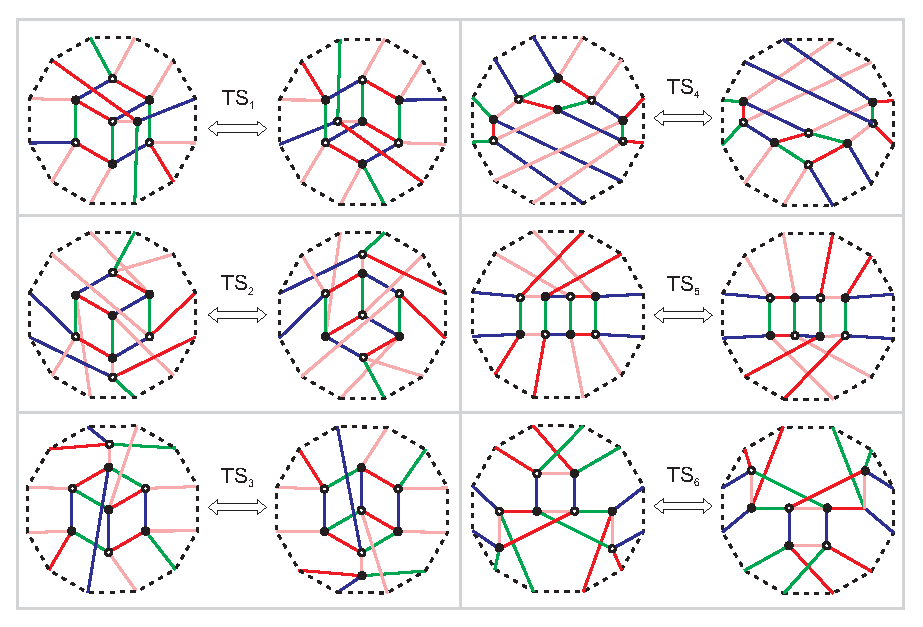
\includegraphics{A.figs/tsmoves.eps}\\
   \end{center}
   \vspace{-0.7cm}
   \caption{The six TS-moves}
   \label{fig:tsmoves}
   \vspace{-0.5cm}
\end{figure}

A {\em monopole}\index{monopole} in a $(3+1)$-graph is a vextex
which is the only intersection of an $hi$-gon and a $jk$-gon,
$(h,i,j,k)$ a permutation of $(0,1,2,3)$. This defines a
configuration which induces a fundamental move in the classification
of gems. A $U_{mn}$-move is defined on a monopole, by making the
$hi$-gon of size $2m$ and the $jk$-gon of size $2n$ (whose union has
$2m+2n-1$ vertices) disappear, being replaced by a cluster of
squares with $(2m-1) \times (2n-1)$ vertices. A $U_{mn}$-move does
not change the induced space of the gem. We give an example in
Figure~\ref{fig:umove} of $U_{23}$ move. In general the
$U_{mn}$-move increases the number of vertices of a gem. However, in
conjuntion with the TS-moves and $\rho$-pairs the $U_{mn}$-moves
have been so far sufficient to classify gems up to 30 vertices.

\enlargethispage{2cm}

\begin{figure}[htp]
   \begin{center}
      \leavevmode
      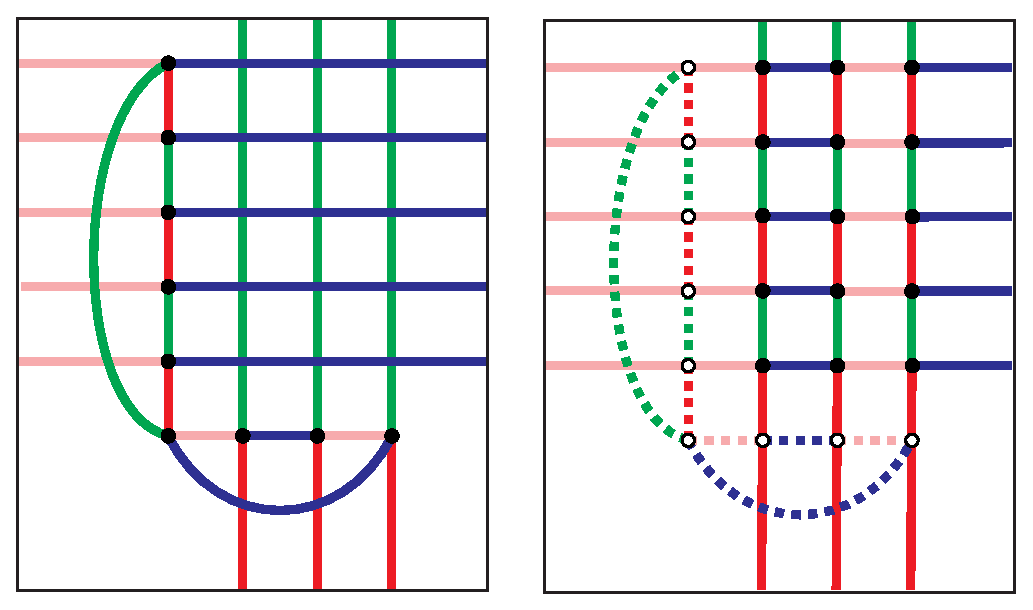
\includegraphics[width=10cm]{A.figs/umove.eps}\\
   \end{center}
   \vspace{-0.7cm}

  \caption{$U_{2,3}$-move applied to a
  1-monopole of type (2,3)}
  \label{fig:umove}
\end{figure}

\newpage

\section{From g-blink to 3-gem}
\label{sec:fromGBlinkTo3Gem}

Assume that $G$ is a g-blink with no g-zigzags with g-edges
alternating red and green. This kind of g-zigzag corresponds in the
BFL to a component that goes totally over or totally under and can
be separated from the rest of the BFL by Reidemeister moves $II$ and
$III$. Assume the following convention on the colors of a gem: $0
\equiv$ pink, $1 \equiv$ blue, $2 \equiv$ red, $3 \equiv$ green. We
begin by proving a result which simplifies considerably the passage
``blink $\rightarrow$ gem'' first given in
\cite{KauffmanAndLins1994}.

\begin{figure}[htp]
   \begin{center}
      \leavevmode
      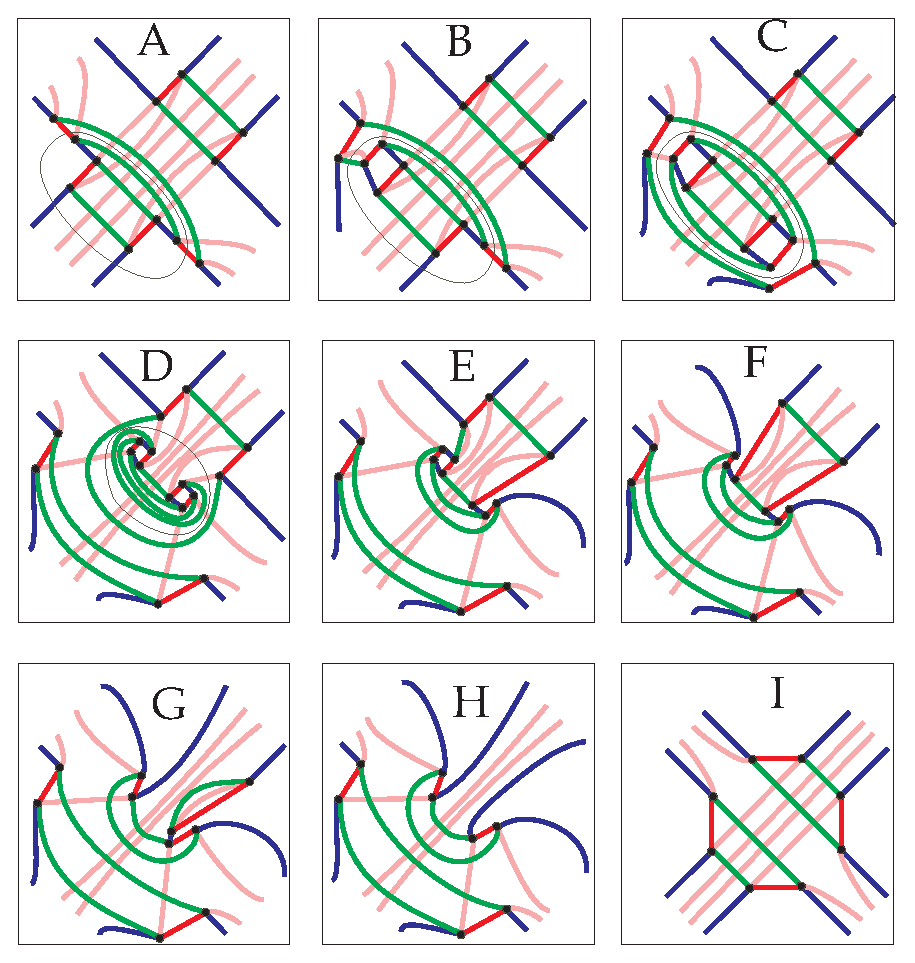
\includegraphics[width=10cm]{A.figs/the-12-8-move.eps}\\
   \end{center}
   \vspace{-0.7cm}
   \caption{Simplifying the gem of a blink: from 12 to 8 vertices by crossing}
   \label{fig:The12x8Move}
\end{figure}

\begin{Theo} \label{theo:blinkToGem}
Given a g-blink $B$ with no alternating g-zigzags it is possible to
obtain a gem $J^\downarrow$ where each edge of the blink (which
corresponds to a crossing of the associated BFL) becomes the
sub-configuration of $8$ vertices shown in Figure~\ref{fig:The12x8Move}I
so that $B$ and $G(B)$ induce the same
space.
\end{Theo}
\begin{proof}
It is proved in \cite{KauffmanAndLins1994} that replacing each
crossing of the BFL associated to the blink by the configuration of
Figure~\ref{fig:The12x8Move}A the final gem $J^\downarrow$ will have
the desired property. The rest of the proof consists in effecting
dipole moves in $J'$ so as to arrive at $J$. The sequence of dipole
moves are depicted in Figure \ref{fig:The12x8Move}. The dipole
moves are local and should be made in the neighborhood of each
original crossing of the BFL. The resulting gem is $J^\downarrow$.
\end{proof}




The gem obtained from a blink by replacing each color of the BFL by
the configuration of Figure \ref{fig:The12x8Move}I is called the
{\em reduced canonical gem} of the blink.

We introduce the following notation to represent both a crossing and
its switched form. The {\em octagon} of a crossing corresponds to an
unidentified crossing. This is indicated by light green edges in the
place of the normal green ones.
\begin{center}
      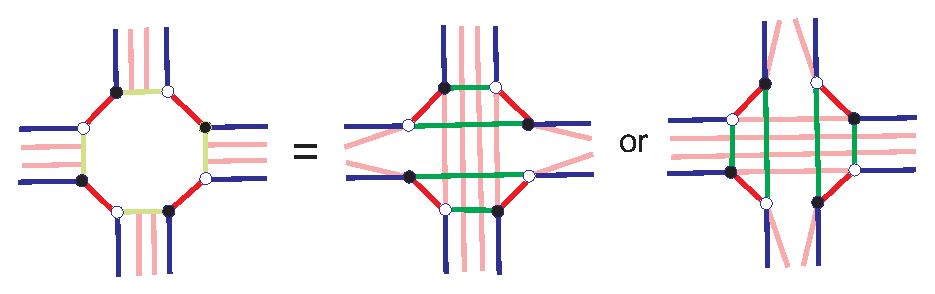
\includegraphics[width=10cm]{A.figs/thetwocrossings.eps}
\end{center}

In Figure \ref{fig:poincareGemBlink} we display a complete example
of the above algorithm to go from a blink $B$ to its canonical gem
$J(B)$ inducing the same space. This example corresponds to
Poincar�'s homology sphere. Observe that an immersion of the gem in
the plane is directly obtained from the embedding of the BFL. The
gem obtained is bipartite. In going clockwise along the
(blue,red)-gons (which corresponds to the faces of the BFL) the red
edges go from a black to a white vertex. Observe that the pink-green
gons form a neighborhood of the original blink. The convention here
is that the green edges are the overpasses, while the pink edges the
underpasses.

\begin{figure}[htp]
   \begin{center}
      \leavevmode
      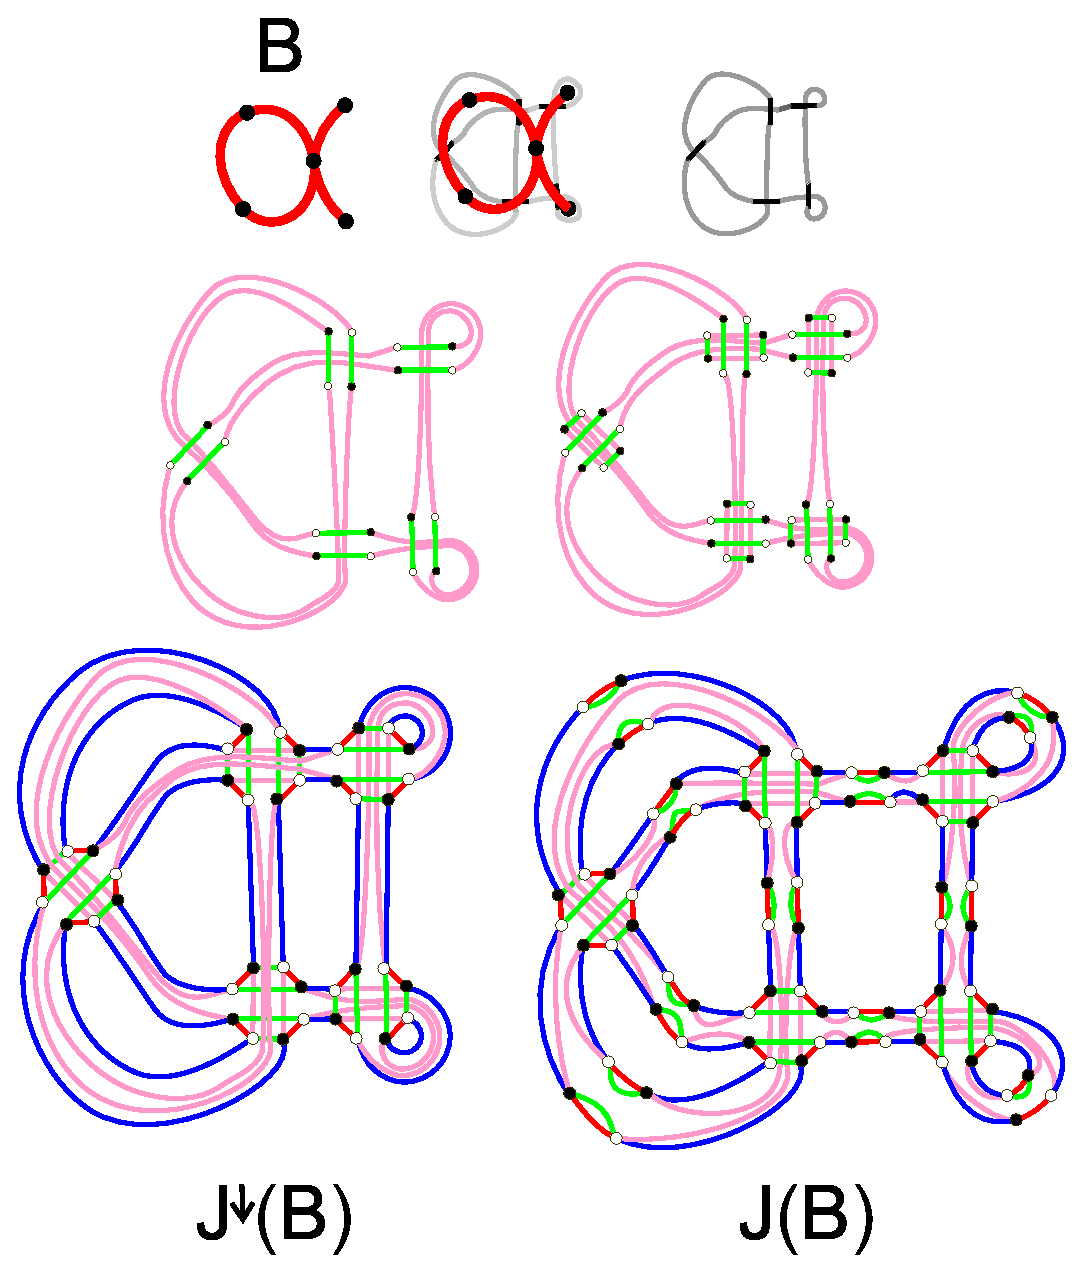
\includegraphics[width=15cm]{A.figs/poincaregemblink.eps}
   \end{center}
   \vspace{-0.7cm}
   \caption{ Obtaining the canonical gems $J^\downarrow(B)$ and
   $J(B)$ from a blink $B$}
   \label{fig:poincareGemBlink}
\end{figure}

The difference between the {\em canonical reduced} gem of the blink
$J^\downarrow(B)$ and the {\em canonical} gem of the blink $J(B)$ is
that we introduce in the latter two 2-dipoles (red-green digons) at
each site corresponding to a g-edge of the original g-blink. While
redundant these $4|E(B)|$ vertices are convenient for our purposes
as we show next. In the computer implementation we use only
$J^\downarrow(B)$. The construction of
Figure~\ref{fig:poincareGemBlink} emphasizes the geometric
simplicity of the algorithm.

The main point in using the auxiliary red-green digons in defining
$J=J(B)$ is that they induce, for each directed g-edge $e$ between
crossings $\alpha$ and $\gamma$, three cylinders $\C_e, \C_\alpha,
\C_\gamma$. For a color $i$ and a vertex $a$ of a gem, denote by
$a_i$ the $i$-colored edge incident to $a$. Let $a_i^\star$ denote
the $2$-simplex in the dual pseudo-complex $J^\star$ corresponding
to the edge $a_i$ of the gem $J$.

\begin{Lem} Let $q,r,s,t$ be the ends of the two
red-green digons induced in $J$ by the directed edge $e$ of $B$, as
shown in Figure~\ref{fig:cylinderInEdge}. Then the sub-complex
$\C_e=q_2^\star + q_3^\star + r_1^\star + r_0^\star$ is a
non-singular cylinder in $J^\star$.
\end{Lem}
\begin{proof}
Two $2$-simplexes of $J^\star$ in colors $i$ and $j$ have a common
$1$-simplex if and only if the dual edges are in the same
$(i,j)$-gon. Note that $q_2$ and $q_3$ are in the same $(2,3)$-gon,
$q_3$ and $r_1$ are in the same $(3,1)$-gon, $r_1$ and $r_0$ are in
the same $(1,0)$-gon and $r_0$ and $q_2$ are in the same
$(0,2)$-gon. To complete the proof just note that there are $4$
distinct vertices in the subcomplex $\C_e$, that $q_2$ and $r_1$ are
not in the same $(2,1)$-gon and finally, that $q_3$ and $r_0$ are
not in the same $(3,0)$-gon.
\end{proof}


The cylinder $\C_e$ is contained in the dual pseudo-complex
$J^\star(B)$. Take a neighborhood $\C_e \times [0,\epsilon]$ in
$|J|$ identify $\C_e \times \{\epsilon/2\}\equiv \C_e$ and define
$\C_\alpha = \C_e \times \{0\}$ and $\C_\gamma = \C_e \times
\{\epsilon\}$. Let $K$ be a simplicial complex which is a refinement
of $J^\star$ containing both $\C_\alpha$ and $\C_\gamma$ as
sub-complexes. We observe that $|J|=|J^\star|=|K|$ and that
vertices $r$ and $s$ of gem $J$ are in $\C_e \times [0,\epsilon]$.


\begin{figure}[htp]
   \begin{center}
      \leavevmode
      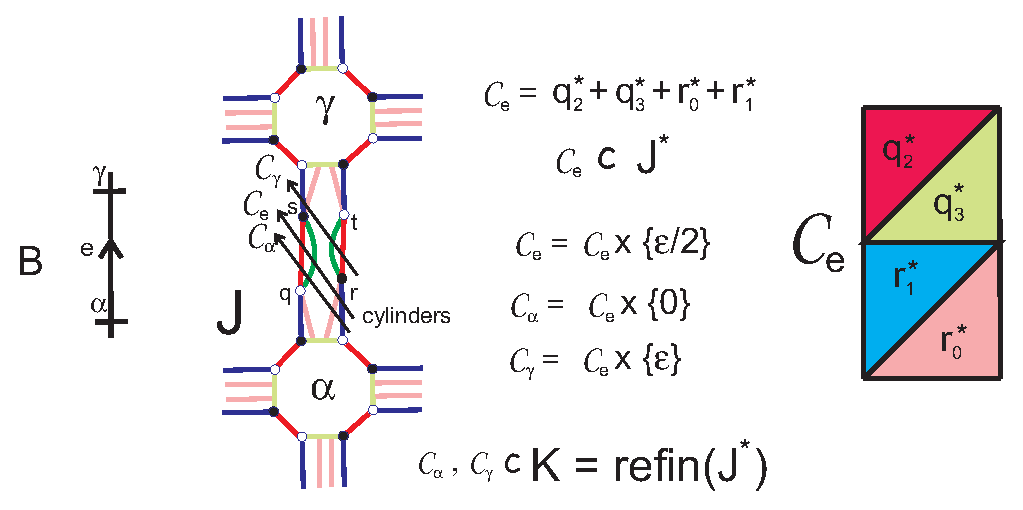
\includegraphics[width=12cm]{A.figs/cylinderinedge.eps}
   \end{center}
   \vspace{-0.7cm}
  \caption{Some cylinders induced in $K(B)$ by a directed
  edge of the BFL between crossings $\alpha$ and $\gamma$}
  \label{fig:cylinderInEdge}
\end{figure}

The procedure \textsc{GBlink2Gem} that follows apply to g-blinks
without alternating zigzags. The procedure is purely combinatorial
and it teaches the computer to go from a g-blink $G$ to the 3-gem
$J^\downarrow$ given in Theorem \ref{theo:blinkToGem}. For each
vertex $v$ of $G$ we define two vertices $v_i$ and $v_o$ in $j$.
\begin{figure}[htp]
   \begin{center}
      \leavevmode
      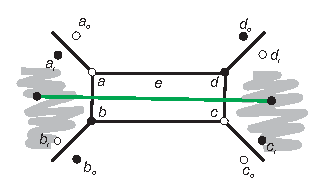
\includegraphics{A.figs/gblink2gem.eps}
   \end{center}
   \vspace{-0.7cm}
   \caption{ Scheme to define a 3-gem from a g-blink}
   \label{fig:gBlink2gem}
\end{figure}
Let $e$ be a g-edge on $G$ with vertices $a, b, c, d$ as shown in
Figure~\ref{fig:gBlink2gem}. Note that $(a,b)$ and $(c,d)$ are
face-edges and $(a,d)$ and $(b,c)$ are vertex-edges. The vertices
$a_i$, $a_o$, $b_i$, $b_o$, $c_i$, $c_o$, $d_i$, $d_o$ of
$J^\downarrow$ corresponding to $a$, $b$, $c$, $d$ are also shown on
Figure~\ref{fig:gBlink2gem}. The $i$ (in) index indicates that the
vertex is drawn inside a g-vertex and the $o$ (out) index indicates
that the vertex must be drawn inside a g-face (or outside the
g-vertex). The edges of $J^\downarrow$ are defined according to the
following procedure:
\begin{enumerate}
\item Each g-edge $e$ of $G$ aligned like the scheme of
Figure~\ref{fig:gBlink2gem} induce the following
edges~on~$J^\downarrow:$
\begin{center}
\begin{small}
\begin{tabular}{l|p{2.7cm}|p{2.7cm}|p{2.7cm}|p{2.7cm}} \hline
& color 0 & color 1 & color 2 & color 3 \\[0.1cm] \hline
   $e$ is green &
   $(a_i,c_o)$, $\,\,(a_o,c_i)$ &
   &
   $(a_i,b_i)$, $\,(c_o,b_o)$, $\,(c_i,d_i)$, $\,(d_o,a_o)$ &
   $(a_i,a_o)$, $\,(b_i,d_o)$, $\,(b_o,d_i)$, $\,(c_i,c_o)$
   \\[0.1cm] \hline
   $e$ is red &
   $(b_i,d_o)$, $\,(b_o,d_i)$ &
   &
   $(a_i,b_i)$, $\,(c_o,b_o)$, $\,(c_i,d_i)$, $\,(d_o,a_o)$ &
   $(a_i,c_o)$, $\,(b_i,b_o)$, $\,(a_o,c_i)$, $\,(d_i,d_o)$
   \\[0.1cm] \hline
\end{tabular}
\end{small}
\end{center}
\item For every angle-edge $\hat{e} = (u,v)$ in $G$ edges
$(u_i,v_i)$ and $(u_o,v_o)$, both with color 1, are added to
$J^\downarrow$.
\newpage

\item At this point, some vertices in $J^\downarrow$
do not have a color 0 incident edge. Let $u$ be a vertex in
$J^\downarrow$ without a neighbor of color 0. We add the edge
$(u,v)$ with color 0 in $J^\downarrow$, where $v$ is the result of
$$
\begin{array}[t]{l}
x \leftarrow {\rm neighbor}(v,1) \\
c \leftarrow 0 \\
\hbox{\bf while } {\rm neighbor}(x,c) \hbox{ is defined} \\
\hspace{1cm} x \leftarrow {\rm neighbor}(x,c) \\
\hspace{1cm} c \leftarrow (c + 1) \,\, {\rm mod} \,\, 2\\
v \leftarrow x \\
\end{array}.
$$
The expression ${\rm neighbor}(x,c)$ denotes the vertex adjacent to
$x$ by color $c$ in $J^\downarrow$. We do this until every vertex
has an incident color 0 edge.
\end{enumerate}
According to Theorem~\ref{theo:blinkToGem}, $J^\downarrow$ defined
this way is a 3-gem and it induces the same space as $G$ does. We
denote this procedure described here as \textsc{GBlink2Gem}. A
complete example of a g-blink and the 3-gem defined by
\textsc{GBlink2Gem} is depicted on Figure~\ref{fig:gBlinkAndGem}.
\begin{figure}[htp]
   \begin{center}
      \leavevmode
      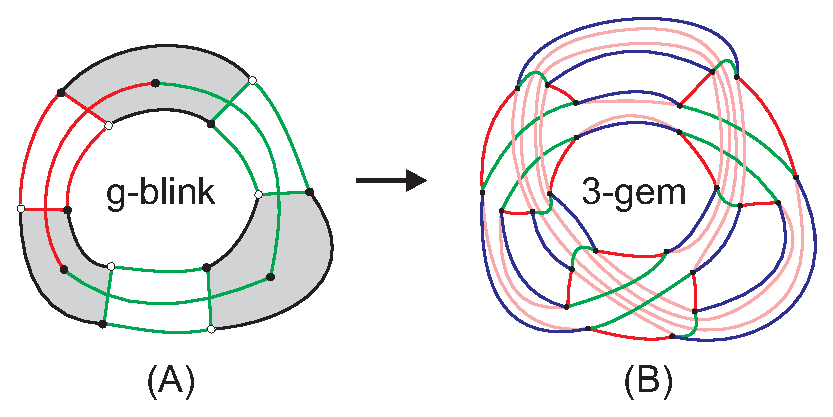
\includegraphics[width=9cm]{A.figs/gblinkandgem.eps}
   \end{center}
   \vspace{-0.7cm}
   \caption{ g-blink $G$ and its reduced canonical
   3-gem $J^\downarrow(G)$ defined by \textsc{GBlink2Gem}}
   \label{fig:gBlinkAndGem}
\end{figure}

\newpage
\section{A proof of the partial reflection theorem}
\label{sec:proofOfThePartialReflectionTheorem}
We first show that a breakpair $\{e,f\}$ in a g-blink $C$
corresponds in $J^\star=J^\star(C)$ to a separating non-singular
$2$-torus $T^2_{ef}$.

\begin{figure}[htp]
   \begin{center}
      \leavevmode
      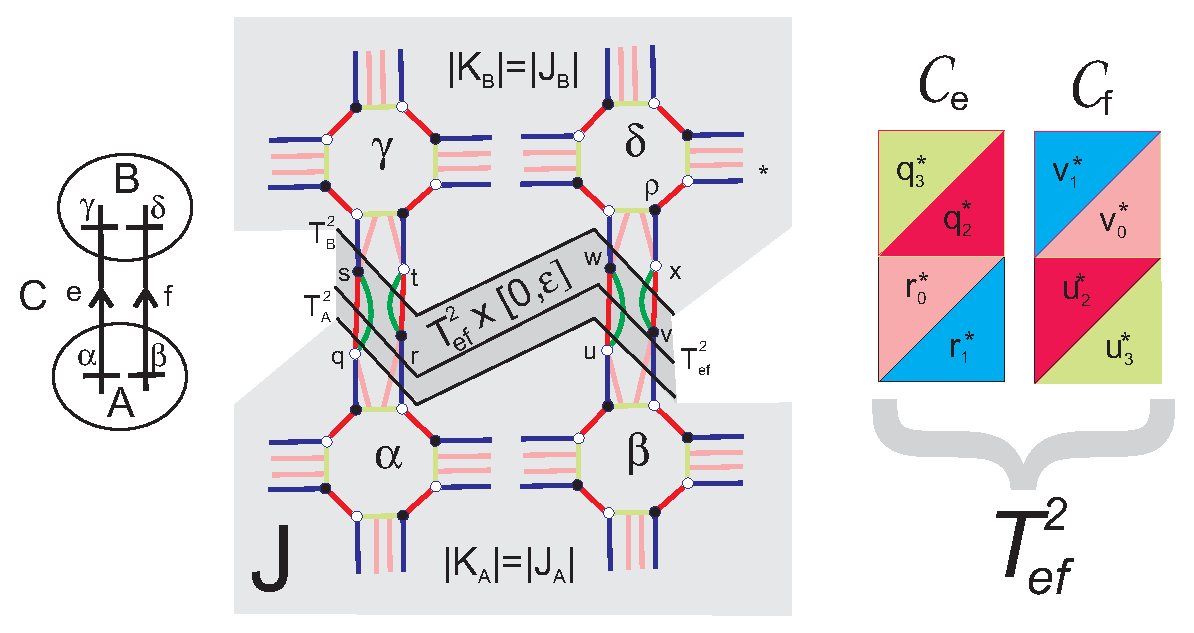
\includegraphics[width=14cm]{A.figs/breakpairandtorus.eps}\\
   \end{center}
   \vspace{-0.7cm}
  \caption{$1-1$ correspondence: breakpair $\{e,f\}$
  in g-blink $C$ $\leftrightarrow$
  separating 2-torus $T_{ef}^2$ in $J^\star=J^\star(C)$ }
  \label{fig:breakpairAndTorus}
\end{figure}


\begin{Lem} \label{lem:torus}
The subcomplex $T^2_{ef} = \C_e + \C_f$ is a non-singular separating
torus in the dual pseudo-complex $J^\star$.
\end{Lem}

\begin{proof} We have seen already that $\C_e$ and $\C_f$ are
cylinders in $J^\star$. It remains to show that these cylinders have
the same boundary and that $\C_e + \C_f$ is a torus. We refer to
Figure~\ref{fig:breakpairAndTorus}. Note that $q_2$ and $v_1$ are in
the same $(2,1)$-gon, $r_1$ and $u_2$ are in the same $(1,2)$-gon,
$q_3$ and $v_0$ are in the same $(3,0)$-gon and that $r_0$ and $u_3$
are in the same $(0,3)$-gon. So, $T^2_{ef}=\C_e + \C_f$ is a
non-singular torus. It clearly separates. This completes the proof.
\end{proof}

To simplify the notation henceforth we write $T^2$ in place of
$T^2_{ef}$. Consider an $\epsilon$-neighborhood $T^2 \times
[0,\epsilon]$ of $T^2 \subset K$ so that $T^2 \equiv T^2 \times
\{\epsilon/2\}$. If we now remove $T^2 \equiv T^2 \times
\{0,\epsilon\}$ from $|K|$ then we have two disjoint spaces $|K_A|$
with boundary $\C_\alpha + \C_\beta = T_{\alpha\beta}^2 \equiv T^2
\times \{0\}$ and  $|K_B|$ with boundary $\C_\gamma + \C_\delta =
T_{\gamma\delta}^2 \equiv T^2 \times \{\epsilon\}$ as shown in
Figure~\ref{fig:breakpairAndTorus}. It follows that
\begin{equation}\label{eq:tripartition1} |K| = |K_A| \cup \left(T^2
\times [0,\epsilon]\right)\ \cup\ |K_B|,\end{equation} with
\begin{equation}\label{eq:tripartition2} |K_A| \cap \left(T^2 \times
[0,\epsilon]\right) = T_{\alpha\beta}^2 , \hspace {8mm} \left(T^2
\times [0,\epsilon] \cap |K_B| \right) = T^2_{\gamma\delta}, \hspace
{8mm} |K_B| \cap |K_A| = \emptyset.\end{equation}

For the proof of the Partial Reflection Theorem we present the
$2$-torus as the quotient space of $\IR^2$ by the lattice of integer
points: $T^2={\frac{\IR\times \IR}{\IZ\times \IZ}}$. Seeing $T^2$ in
this way, the $\pi$-rotational symmetry that we will need becomes
simply $(x,y) \mapsto (-x,-y)$. Let $F = \IR\times \IR \times
[0,\pi]$. Consider the auto-homeomorphism $\mu$ of $F$ given by
$$\mu(x,y,\theta)=\left(x\, \cos\, \theta
+y\, \sin\, \theta, -x\, \sin\, \theta+y\, \cos\, \theta,\,
\theta\right).$$

Define $\equiv'$ as the equivalence relation on $F$: $(x,y,\theta)
\equiv' (x',y',\theta')$ if $\theta'=\theta$, $x-x' \in \IZ$ and
$y-y' \in \IZ$. The quotient space $F / \equiv'$ is denoted by $F'$.
The image under $\mu$ of a the vertical segment linking $(x,y,0)$ to
$(x,y,\pi)$ is a helicoidal curve that starts at $(x,y,0)$, and
finishes at $(-x,-y,\epsilon)$. Note that any two vertical segments
in $F$ whose distance is an integer are identified. Clearly $F'
\approx \IS^1 \times \IS^1 \times [0,\epsilon]$.

Define $\equiv_\mu$ as another equivalence relation on $F$ given by
$$(x,y,\theta) \equiv_\mu (x',y',\theta') {\hspace{5mm}\rm
if \hspace{5mm} } \mu^{-1}(x,y,\theta) \equiv'
\mu^{-1}(x',y',\theta'), \rm {\ that\ is,\ if \ } \theta=\theta'
\rm{\ and} $$  $$ x\,\cos\, \theta -y\, \sin\, \theta - x'\, \cos\,
\theta'+ y'\, \sin\, \theta' \in \IZ$$
$$x\, \sin\, \theta + y\,
\cos\, \theta - x'\, \sin\, \theta' - y'\, \cos\, \theta' \in \IZ.$$
The space $F/\equiv_\mu$ is denoted by $\widetilde{F}$. Observe the
simple fact that $\mu$ induces a homeomorphism sending $F'$ onto
$\widetilde{F}$, also named $\mu$ by abuse of language. As a
consequence of our definitions, two helicoidal curves in $F$ are
identified in $\widetilde{F}$ if their pre-images under $\mu$ are
two vertical segments identified in $F'$. The action of $\mu$ in the
fundamental domain centered at the origin from $F'$ to
$\widetilde{F}$ is shown in Figure~\ref{fig:filme}.
\begin{figure}[htp]
   \begin{center}
      \leavevmode
      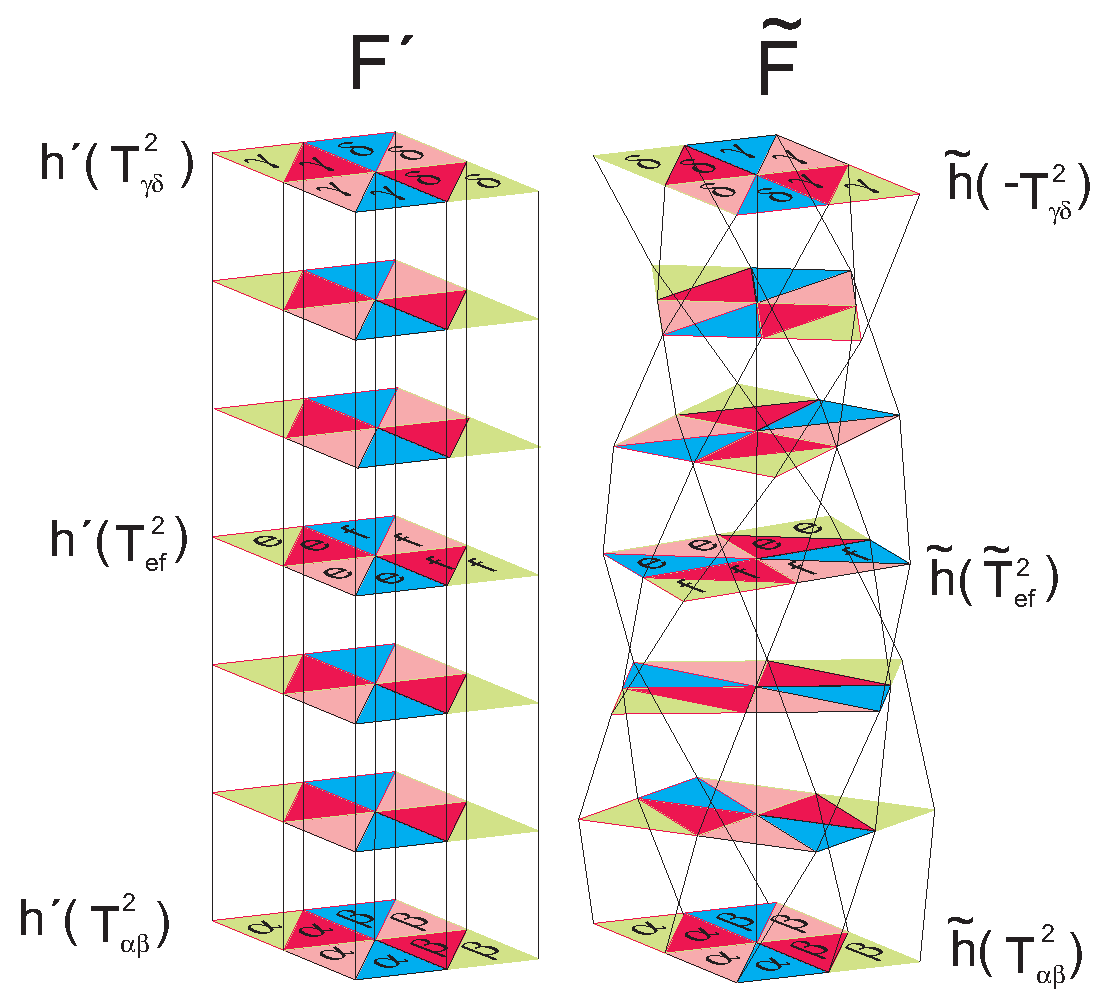
\includegraphics[width=15cm]{A.figs/filme.eps}\\
   \end{center}
   \vspace{-0.7cm}
  \caption{The action of $\mu$ on the fundamental domain
  centered at the origin mapping $F'$ onto $\widetilde{F}$}
  \label{fig:filme}
\end{figure}

We are now ready to prove Theorem~\ref{theo:partialReflection}

\begin{figure}[htp]
   \begin{center}
      \leavevmode
      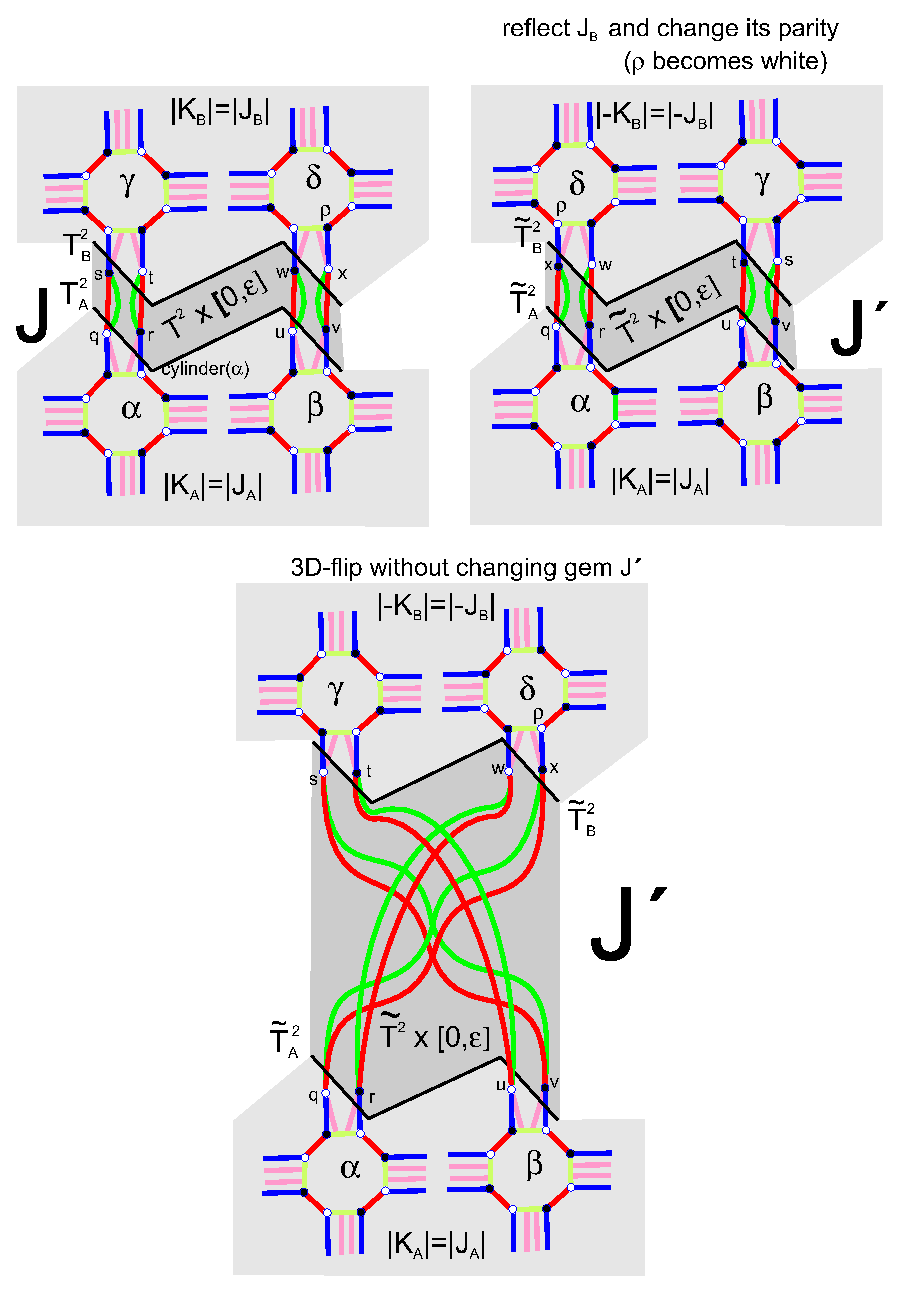
\includegraphics[width=15cm]{A.figs/inthreeparts.eps}\\
   \end{center}
   \vspace{-0.7cm}
  \caption{For the proof of the Partial Reflection Theorem:
  gems $J$ and $J\, '$ induce the same space}
  \label{fig:inThreeParts}
\end{figure}

\noindent {\bf Proof of Theorem~\ref{theo:partialReflection}:\ } Let
$A$ and $B$ be arbitrary disjoint g-blinks, $(a,b)$ a basepair on
them. Then $A[a] + B[b] \Sequiv A[a] + \textsc{Reflection}(B)[b].$
\begin{proof}
Let $J$ be the canonical gem of the g-blink $A[a] + B[b]$ and $J\,
'$ be the canonical gem of g-blink $A[a] +
\textsc{Reflection}(B)[b]$. Let $K$ be a simplicial refinement of
$J^\star$ containing the $2$-torus $T^2$ (given in
Lemma~\ref{lem:torus}) as a subcomplex. Let $\widetilde{K}$ be a
simplicial refinement of $(J')^\star$ containing the $2$-torus
$\widetilde{T^2}$ (which plays in $J'$ the same role of $T^2$ in
$J$) as a subcomplex. Let $h'$ be a fixed homeomorphism which maps
$T^2 \times [0,\epsilon]$ onto $F'$ and $\widetilde{h}$ be a fixed
homeomorphism which maps $\widetilde{T^2} \times [0,\epsilon]$ onto
$\widetilde{F}$. By applying Equations~\ref{eq:tripartition1} and
\ref{eq:tripartition2} to the tori $T^2$ and $\widetilde{T^2}$ we
have ($-K_B$ is $K_B$ with orientation reversed: they are oriented
simplicial complexes):
$$ |K| = |K_A| \cup \left(T^2 \times
[0,\epsilon]\right)\ \cup\ |K_B|, \hspace{3mm} |\widetilde{K}| =
|K_A| \cup \left(\widetilde{T_2} \times [0,\epsilon]\right)\ \cup\
|-K_B|, \hspace{3mm} |K_A| \cap |K_B| = \emptyset.$$ with
\begin{equation}
\label{eq:tripartition4} |K_A| \cap \left( T^2 \times
[0,\epsilon]\right) = T_{\alpha\beta}^2, \hspace {8mm} \left({T^2}
\times [0,\epsilon]\right) \cap |K_B| = T_{\gamma\delta}^2,
\end{equation}
$$ |K_A| \cap \left( \widetilde{T^2} \times
[0,\epsilon]\right) = T_{\alpha\beta}^2, \hspace {8mm} \left(
\widetilde{T^2} \times [0,\epsilon]\right) \cap |-K_B| =
-T_{\gamma\delta}^2.$$ Define the map $\rho$ from $|K|$ to
$|\widetilde{K}|$ to be the identity in $|K_A| \cup |K_B|$. For $x
\in T^2 \times [0,\epsilon]$, define $\rho(x) = \left[(\,
\widetilde{h}\, )^{-1}\ {\circ} \ \mu\ {\circ} \ h'
\right](x) \in \widetilde{T^2} \times [0,\epsilon]$. Map $\rho$ is
the desired homeomorphism taking $|K|$ onto $|\widetilde{K}|$.
\end{proof}

We finish this chapter by proving the following Theorem about BFLs
with a segment between crossings removed:
\begin{Theo} \label{BFLwithSegmentRemoved}
Let $B^\circ$ be a BFL $B$ with a segment between crossings removed.
There exists a well defined 3-manifold with toroidal boundary
$S^\circ$ which can be associated to $B^\circ$. Moreover, there
exists a canonical way to close $S^\circ$ by attaching a solid torus
to its boundary to get a space $S$ such that $|B|=S$.
\end{Theo}
\begin{proof} The proof should be followed in Figure~\ref
{fig:spaceToroidalBoundary}. Gem $J$ is the canonical gem of the BFL
$B$. Gems $J\, '$ and $J\, '\, '$ are obtained from $J$ by 2-dipole
creations. The last gem is subdivided into two gems with boundary
$H$ and $U$. The boundaries of these gems are homeomorphic to the
$2$-torus $T^2_{ef} = \C_e + \C_f$ , given in Lemma~\ref{lem:torus}.
It can be shown that gem with toroidal boundary $U$ induces a solid
torus, thus completing the proof.
\end{proof}

\begin{figure}[htp]
   \begin{center}
      \leavevmode
      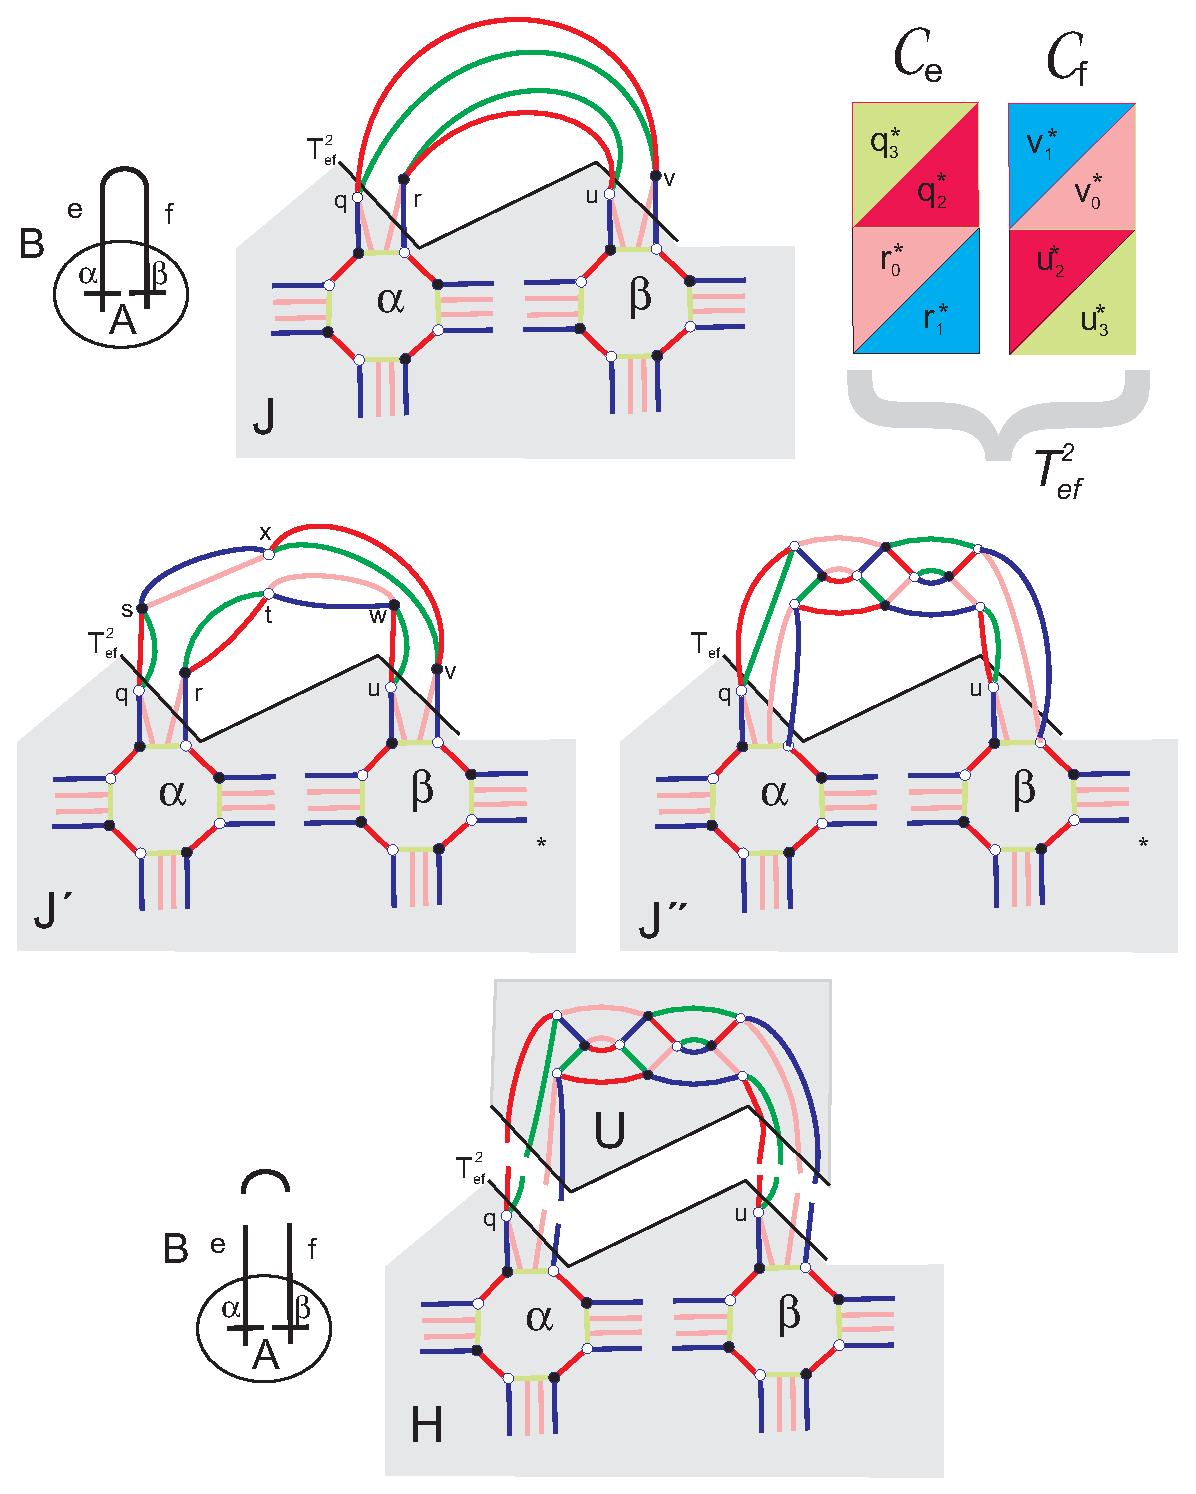
\includegraphics[width=12cm]{A.figs/spacetoroidalboundary.eps}\\
   \end{center}
   \vspace{-0.7cm}
  \caption{Space $|H|$, $\partial(|H|)=T^2_{ef}$, canonical way
  to close it: $|B|=|H| \cup_{T^2_{H}\equiv T^2_U} |U|$, $|U|$ solid torus}
  \label{fig:spaceToroidalBoundary}
\end{figure}
